\documentclass[10pt]{beamer}

\usetheme[progressbar=frametitle]{metropolis}
\usepackage{appendixnumberbeamer}

\usepackage{booktabs}
\usepackage[scale=2]{ccicons}

\usepackage{pgfplots}
\usepgfplotslibrary{dateplot}

\usepackage{xspace}
\newcommand{\themename}{\textbf{\textsc{metropolis}}\xspace}

\usepackage{xmpmulti}

\newcommand{\MM}{\mathbf{M}}
\newcommand{\KM}{\mathbf{K}}
\newcommand{\fM}{\mathbf{f}}
\newcommand{\aM}{\mathbf{a}}
\newcommand{\NM}{\mathbf{N}}
\newcommand{\BM}{\mathbf{B}}
\newcommand{\DM}{\mathbf{D}}

\numberwithin{equation}{subsection}

\title{Numerical simulation of membrane deformation under high-speed load}
\subtitle{QIPA 2018}
% \date{\today}
\date{December 4, 2018}
\author{V. Aksenov, A. Vasyukov, K. Beklemysheva  }
\institute{Moscow Institute of Physics and Technology}
\titlegraphic{\hfill
\includegraphics[height=1.5cm]{logo.png}}
\metroset{block=fill}
\begin{document}

\maketitle

\begin{frame}{Table of contents}
  \setbeamertemplate{section in toc}[sections numbered]
  \tableofcontents[hideallsubsections]
\end{frame}

\section{Introduction}

\begin{frame}[fragile]{Problem overview}
    \begin{figure}
    \begin{minipage}{0.49\textwidth}
    	\noindent\centering{
		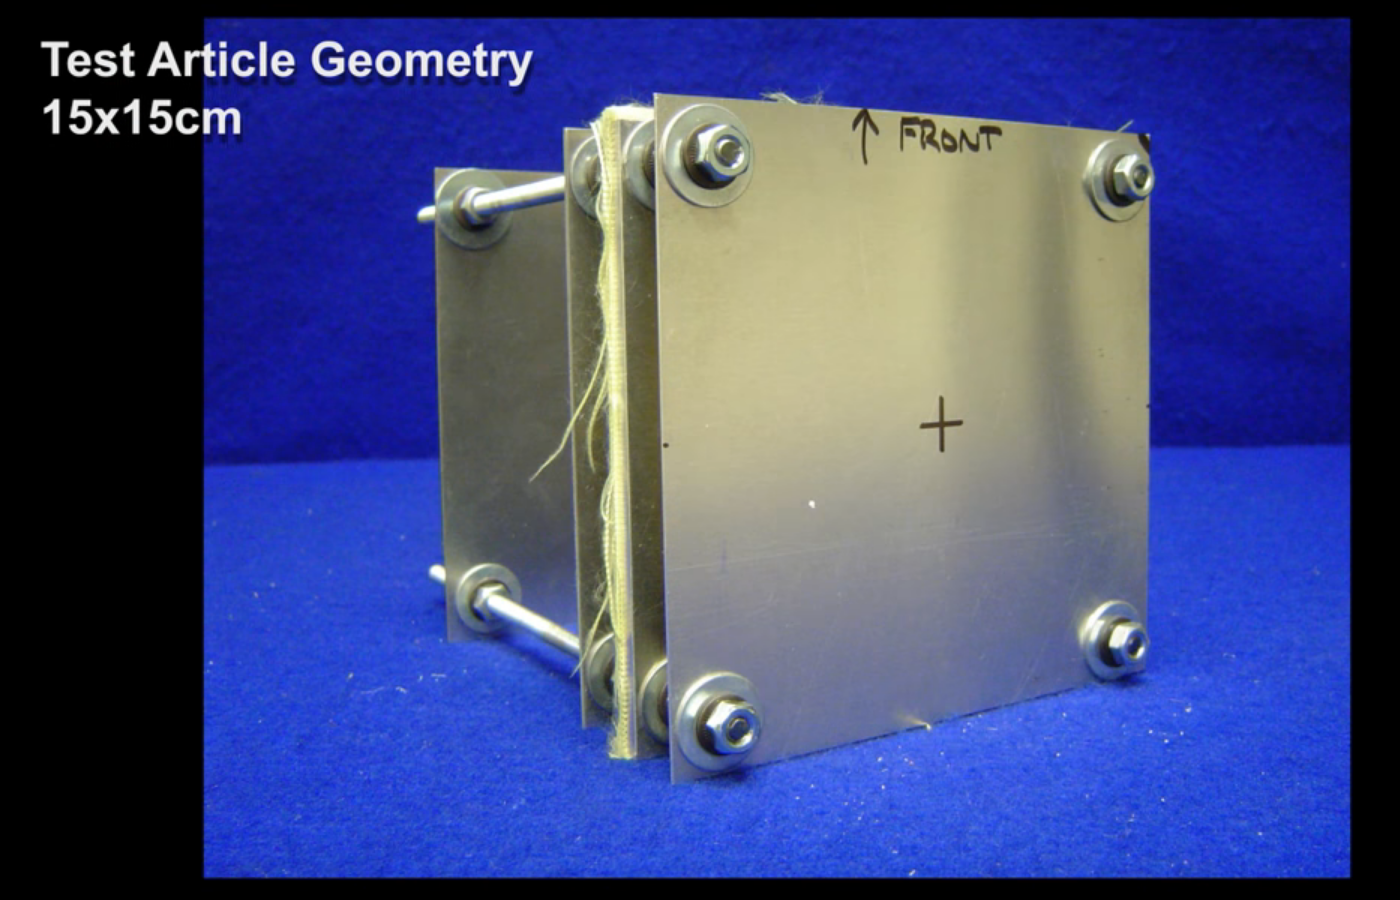
\includegraphics[width=\textwidth]{M1.png}}
        \caption{Protection cover example: two metal layers and textile layer}
	\end{minipage}
    \hfill
    \begin{minipage}{0.33\textwidth}
    	\noindent\centering{
		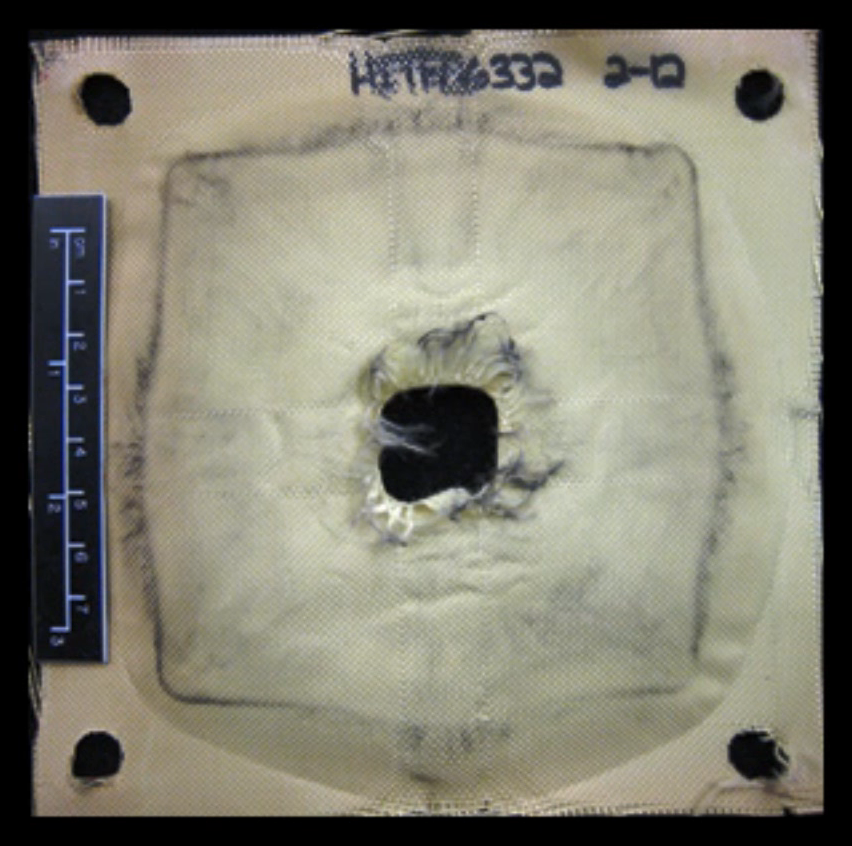
\includegraphics[width=\textwidth]{M2.png}}
        \caption{Textile layer after the impact}
	\end{minipage}
	\end{figure}
	\vfill
	\textbf{Subject area:} meteorite protection for satellites
	\vfill
	\textbf{Scope of current project:}
	\begin{itemize}
	    \item Solving direct problem~---~membrane under high-speed load
	    \item Modeling thin membrane with arbitrary rheology
	    \item Data generation for inverse problem
	\end{itemize}
\end{frame}

\section{Mathematical model}

\begin{frame}{Requirements and assumptions}
    \begin{itemize}
	    \item Thin membrane~---~2D object in 3D space
	    \item Arbitrary load profile, both in time and space
	    \item Large displacements; membrane moves as a whole
    \end{itemize}
\end{frame}

\section{Numerical method}
\begin{frame}{Finite element method (FEM)}
   % Based on \cite{zie00}
   \begin{minipage}{0.60\textwidth}
	\begin{figure}
    	\noindent\centering{
		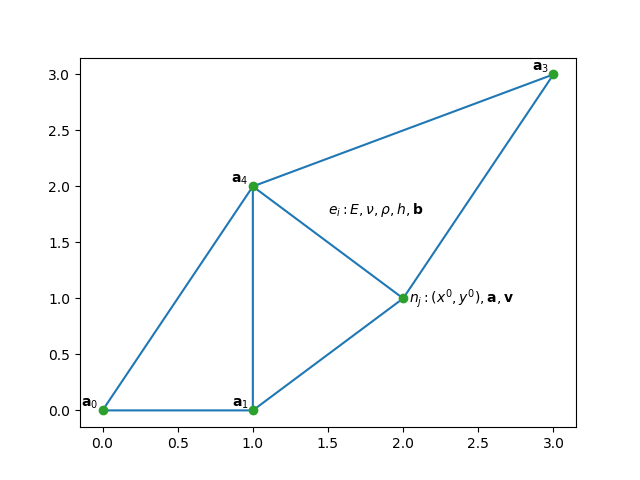
\includegraphics[width=\textwidth]{Div_example.png}}
        \caption{Domain division example; sample element $e_i$ and node $n_j$ with associated values}
	\end{figure}
\end{minipage}
\hfill
\begin{minipage}{0.38\textwidth}
	\begin{enumerate}
       \item Domain division into elements (e.g.~triangles)
       \item Choice of shape functions $\mathbf{u} = \NM\aM$
       \item Reduction to system of algebraic (static) or ordinary differential (dynamic) equations
   \end{enumerate}
\end{minipage}	
   
   
\end{frame}
\begin{frame}{Limitations}
    \begin{itemize}
        \item Only distributed force over an element is considered
        \item Free boundary~---~no constraints or forces on the boundary
        \item Isotropic material
        \item Homogeneous material in element~---~any heterogeneity is accounted for at domain division
    \end{itemize}
    %
    %free border
\end{frame}


\subsection{Element matrices}

\begin{frame}{Shape functions $\mathbf{N}_i^e$}
    Displacements in an element are approximated via \emph{shape~functions}~$\NM_i$:
    \begin{equation}\label{shape}
		\mathbf{u}(x,y,z) = \sum_{i = 1}^3{\mathbf{N_ia_i}} = \mathbf{Na}
	\end{equation}
	where $\NM = \left[ \begin{smallmatrix} \NM_1 & \NM_2 & \NM_3
	                                        \end{smallmatrix} \right]$, 
		$\aM = \left[ \begin{smallmatrix} \aM_1 \\ \aM_2 \\ \aM_3
		                \end{smallmatrix} \right]$~---~nodal displacements.
    \metroset{block=fill}
    \begin{alertblock}{Assumption}
    Displacement doesn't depend on $z$:
        \begin{equation}
			\NM_i = (\alpha_i + \beta_i x + \gamma_i y)\mathbf{E}
		\end{equation}
	as in FEM for $2D$ problems\cite{zie00}
    \end{alertblock}
\end{frame}

\begin{frame}{Strains}
    Writing down strains:
    \begin{equation}
        \varepsilon = \begin{bmatrix}
                        \frac{\partial u}{\partial x} &
                        \frac{\partial v}{\partial y} &
                        \frac{\partial w}{\partial z} &
                        \frac{\partial u}{\partial y} + \frac{\partial v}{\partial x} &
                        \frac{\partial v}{\partial z} + \frac{\partial w}{\partial y} &
                        \frac{\partial w}{\partial x} + \frac{\partial u}{\partial z} 
                    \end{bmatrix}^T
    \end{equation}
	\begin{gather}
		\mathbf{S} =  \begin{bmatrix}
			    	    \mathbf{S}_1 \\
				        \mathbf{S}_2
            	    \end{bmatrix} \notag \\
		\mathbf{S}_1 = \begin{bmatrix}
		                	\frac{\partial}{\partial x}	&	0				&	0	\\	
    						0	                        &  	\frac{\partial}{\partial y}	&	0	\\	
							0	    &	0				&	\frac{\partial}{\partial z}
					    \end{bmatrix} , \quad 
		\mathbf{S}_2 = \begin{bmatrix}
				            \frac{\partial}{\partial y}	&	\frac{\partial}{\partial x}	&	0	\\	
							0	&	\frac{\partial}{\partial z}	&	\frac{\partial}{\partial y}	\\	
				    \frac{\partial}{\partial z}	&	0				&	\frac{\partial}{\partial x}
					    \end{bmatrix} 
	\end{gather}
	\begin{alertblock}{Strains}
        \begin{equation} \label{eps}
	    		\mathbf{\varepsilon} = \mathbf{Su} = \mathbf{SNa} = \mathbf{Ba}
	    \end{equation}	
	\end{alertblock}
	where $\BM$ is the \emph{gradient matrix}
	
\end{frame}

\begin{frame}{Stresses}
    Writing down stresses:
    \begin{equation}\label{stress}
			\mathbf{\sigma} = \begin{bmatrix} 
			                    \sigma_{xx} & 
			                    \sigma_{yy} & 
			                    \sigma_{zz} &
			                    \tau_{xy}   &
			                    \tau_{yz}   &
			                    \tau_{xz}
			                   \end{bmatrix}^T
		\end{equation}
		Assuming isotropic material, let
		\begin{gather}
			\mathbf{D}_1 = \frac{E}{(1 + \nu)(1 - 2\nu)}
				\begin{bmatrix}
					1 - \nu 	& \nu 		& \nu \\
					\nu 		& 1 - \nu  	& \nu \\
					\nu		& \nu		& 1 - \nu
				\end{bmatrix} \\ \notag
			\mathbf{D}_2 = \frac{E}{(1 + \nu)(1 - 2\nu)}
				\begin{bmatrix}
					\frac{1-2\nu}2 	& 0 		& 0 \\
					0 		& \frac{1-2\nu}2& 0 \\
					0		& 0		& \frac{1-2\nu}2
				\end{bmatrix}
		\end{gather}
		\begin{alertblock}{Stresses}
		    \begin{equation}\label{sigma}
		       \sigma = \mathbf{DBa}, \quad 
		       \mathbf{D} = 
				\begin{bmatrix}
					\mathbf{D}_1 	& \mathbf{0}	\\
					\mathbf{0}	& \mathbf{D}_2
				\end{bmatrix} 
			\end{equation}
		\end{alertblock}
\end{frame}

\begin{frame}{Virtual work for the element}
    Let's introduce fictive nodal forces $\mathbf{q}_e$ which are statically equivalent to actual forces. Considering virtual displacements $\delta \mathbf{u}, \delta \mathbf{\varepsilon}$ 
        virtual work per unit volume~is
    \begin{equation}
        \delta w = \delta\mathbf{\varepsilon^T \sigma} - \delta\mathbf{u^t \overline{b}}
    \end{equation}
    \bigskip
    Substituting from~(\ref{shape}),~(\ref{sigma}),~(\ref{eps}) :
    \begin{equation}
        \delta\mathbf{u} = \NM\delta\aM, \quad \delta \mathbf{\varepsilon} = \BM\delta\aM
    \end{equation}
    we get
    \begin{alertblock}{Principle of virtual work}
        \begin{equation}
            \delta \aM^T  \left(\int_{V_e}\mathbf{B^T D Ba}dV
                        - \int_{V_e} \mathbf{N^T\overline{b}}dV \right) = \delta\aM^T\mathbf{q}_e
        \end{equation}
    \end{alertblock}
\end{frame}

\begin{frame}{Stiffness, mass and load matrices $\KM_e, \mathbf{M}_e, \mathbf{f}_e$}
   Dynamic state can be considered as static with added inertial force~$-\rho \ddot{\mathbf{u}}$ (d'Alembert's principle). Substituting 
   \begin{equation}
       \bar{\mathbf{b}} = \mathbf{b} - \rho\ddot{\mathbf{u}},
   \end{equation}
   where $\mathbf{b}$ is actual distributed force, and assuming $\ddot{\mathbf{u}} = \mathbf{N}\ddot{\aM}$
   we get
   \begin{alertblock}{Element matrices}
   \begin{equation}
        \MM_e\ddot{\aM} + \KM_e\aM + \fM_e = \mathbf{q}_e
   \end{equation}
   \begin{gather}
        \KM_e = \int_{V_e}{\mathbf{B^TDB}}dV
            \text{~---~stiffness matrix}\\
        \MM_e = \rho\int_{V_e}{\mathbf{N^TN}}dV
            \text{~---~mass matrix}\\
        \fM_e = - \int_{V_e} \mathbf{N^Tb}dV_e 
            \text{~---~load matrix}
   \end{gather}
   \end{alertblock}
\end{frame}



\subsubsection{Global matrices}
\begin{frame}{Global matrices $\mathbf{K}, \mathbf{M}, \mathbf{f}$}
    Now equations for each element should be \alert{assembled} to acquire equations for the whole domain. Fictive nodal forces 
    $\mathbf{q}=0$,~so:
    \begin{alertblock}{Global matrices}
        \begin{equation}
            \MM\ddot{\mathbf{a}} + \KM\aM + \fM = 0
        \end{equation}
        \begin{gather}
            \KM_{ij} = \sum_{e}\KM^e_{ij} \\
            \MM_{ij} = \sum_{e}\MM^e_{ij} \\
            \fM_i = \sum_{e}\fM^e_{i}
        \end{gather}
    \end{alertblock}
    Here summation is considered over all elements in which $i$ and $j$ are included together, 
    $K_{ij}$ meaning a $3\times3$ block in global $3N_{nodes}\times3N_{nodes}$ matrix, corresponding to $i$-th and $j$-th nodes.
\end{frame}

\begin{frame}{Time integtation}
The problem has been reduced to a $2$-nd order system of ODEs
    \begin{equation*}
        \MM\ddot{\mathbf{a}} + \KM\aM + \fM = 0
    \end{equation*}
We shall integrate it using Newmark~$\beta$-method:
    \begin{gather}
        \dot{\overline{\aM}}_n = \dot{\aM}_n + \tau(1-\beta_1)\ddot{\aM}_n \notag\\
        \overline{\aM}_n = \aM_n + \tau\dot{\aM}_n 
                + \frac12\tau^2(1 - \beta_2)\ddot{\aM}_n \notag\\
        \ddot{\aM}_{n+1} = - A^{-1}\left(\fM_{n+1} +\KM\overline{\aM}_n
                        \right),\quad A = \MM + \frac{1}{2}\tau^2\beta_2\KM\\
        \dot{\aM}_{n+1} = \dot{\overline{\aM}}_n + \beta_1\tau\ddot{\aM}_{n+1} \notag\\
        \aM_{n+1} = \overline{\aM} + \frac{1}{2}\tau^2\beta_2\ddot{\aM}_{n+1} \notag
    \end{gather}
\vspace{-8pt}
\begin{alertblock}{Method properties}
    \begin{itemize}
        \item If $\beta_2 \geq \beta_1 \geq \frac12$ the method is stable regardless of timestep $\tau$
        \item If $\beta_1 = \frac{1}{2}$, the method is second-order accurate \cite{newmark1959method}
        \end{itemize}
    \end{alertblock}
\end{frame}

\section{Simulation results}
\subsection{Simulations}

\begin{frame}{Normal strike}
    \begin{minipage}{0.6\textwidth}
        \begin{figure}\label{norm15tau}
    	\noindent\centering{
		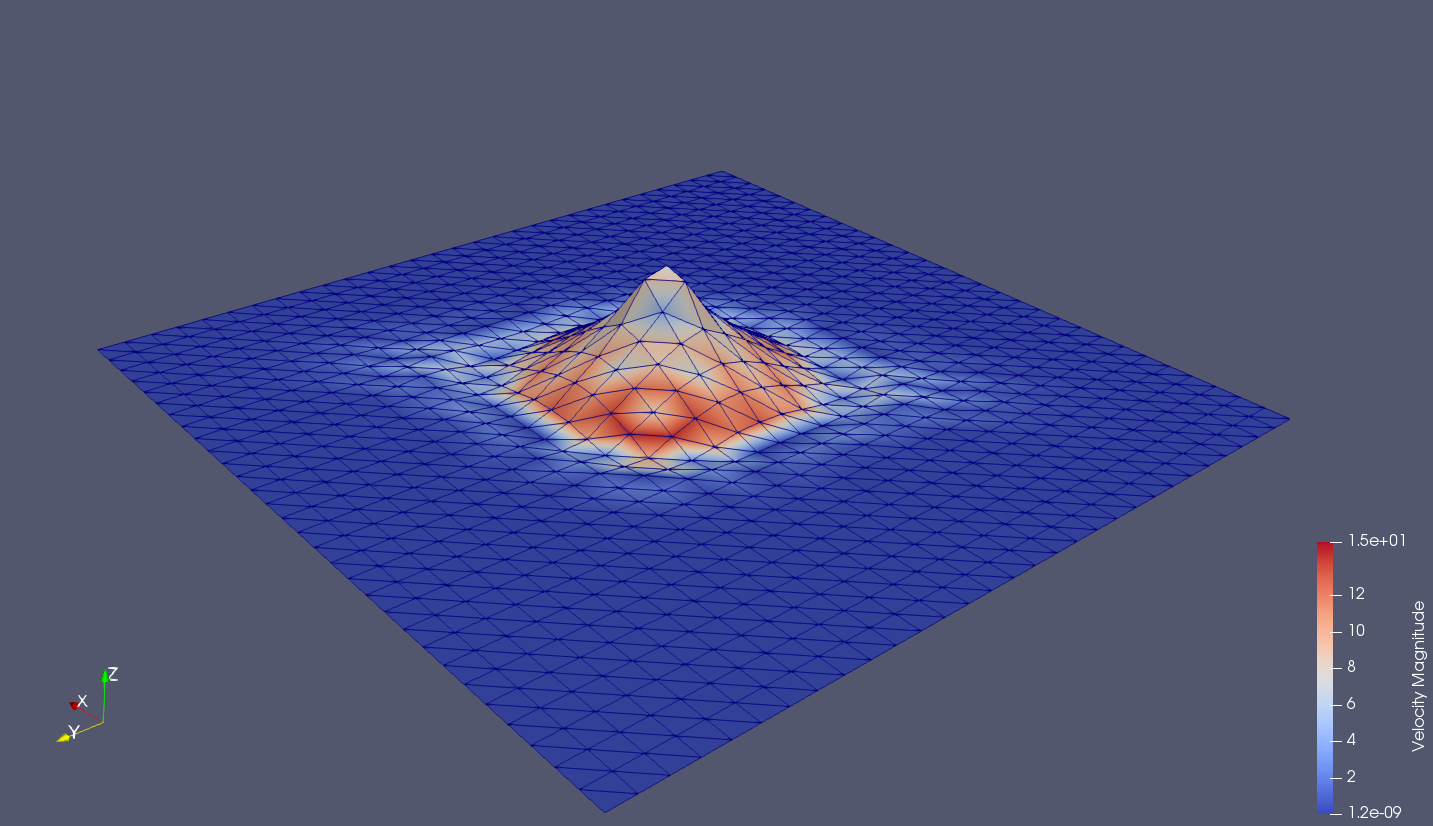
\includegraphics[width=\textwidth]{animation/norm/screen-15.png}}
        \caption{Deformed state at timestep $15\tau$}
	\end{figure}
    \end{minipage}
    \hfill
    \begin{minipage}{0.35\textwidth}
    \begin{tabular}[h]{|l|c|}
\hline
\multicolumn{2}{|c|}{Material properties}\\
\hline
$E,\ MPa$ & $ 1.0$ \\ 
$\nu$ & $ 0.45$ \\ 
$\rho,\ \frac{g}{cm^3}$ & $ 0.9$ \\ 
$h,\ mm$ & $ 1.0$ \\
\hline
\multicolumn{2}{|c|}{Model parameters}\\ 
\hline
$\tau, s$ & $ 1.0\cdot 10^{-4}$ \\ 
Nodes & $31\times31$ \\ 
Size, $m$ & $ 1.0 \times  1.0$ \\
Pressure, $Pa$ & $2.0\cdot10^{5}$ \\
\hline
\end{tabular}
    \end{minipage}
\end{frame}

\begin{frame}{Normal strike}
    \transduration<0-5>{0}
    \multiinclude[<+->][format=png, graphics={width=\textwidth}]{animation/norm/frame}
\end{frame}

\begin{frame}{Skew strike}
    \begin{minipage}{0.6\textwidth}
        \begin{figure}\label{norm15tau}
    	\noindent\centering{
		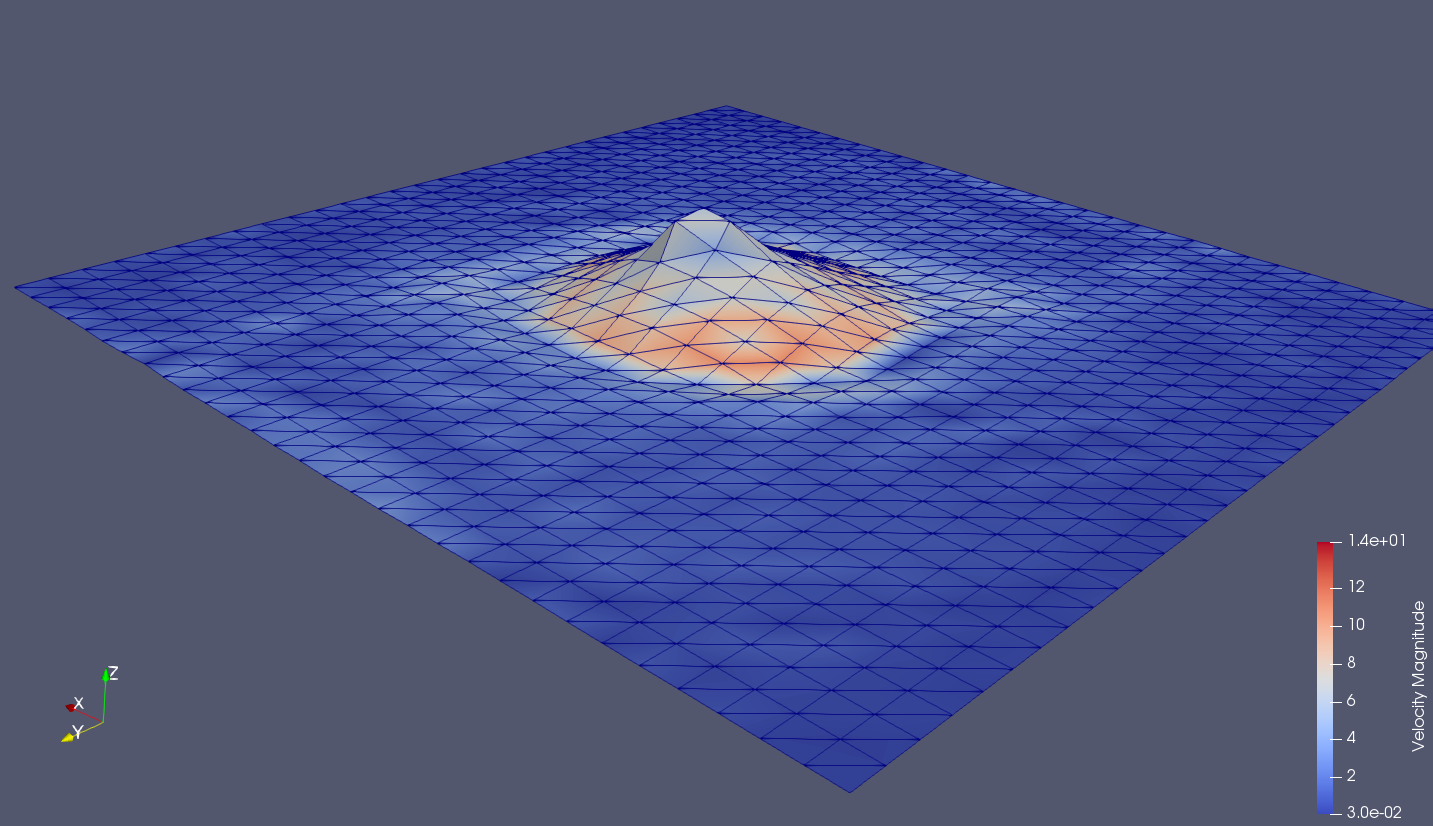
\includegraphics[width=\textwidth]{animation/skew/screen-15.png}}
        \caption{Deformed state at timestep $15\tau$, strike is $45^\circ$ to normal}
	\end{figure}
    \end{minipage}
    \hfill
    \begin{minipage}{0.35\textwidth}
    \begin{tabular}[h]{|l|c|}
\hline
\multicolumn{2}{|c|}{Material properties}\\
\hline
$E,\ MPa$ & $ 1.0$ \\ 
$\nu$ & $ 0.45$ \\ 
$\rho,\ \frac{g}{cm^3}$ & $ 0.9$ \\ 
$h,\ mm$ & $ 1.0$ \\
\hline
\multicolumn{2}{|c|}{Model parameters}\\ 
\hline
$\tau, s$ & $ 1.0\cdot 10^{-4}$ \\ 
Nodes & $31\times31$ \\ 
Size, $m$ & $ 1.0 \times  1.0$ \\
Pressure, $Pa$ & $2.0\cdot10^{5}$ \\
\hline
\end{tabular}
    \end{minipage}
\end{frame}

\begin{frame}{Skew strike}
    \transduration<0-5>{0}
    \multiinclude[<+->][format=png, graphics={width=\textwidth}]{animation/skew/frame}
\end{frame}


\subsection{Results overview}
\begin{frame}{Results overview}
    \begin{itemize}
        \item Deformation cone for isotropic material model (instead of deformation cross obtained in related works based on pure textile membrane model)
        \item Model can be generalized to handle anisotropic materials with arbitrary anisotropy type
        \item Model handles large displacements and membrane movement as~a~whole
    \end{itemize}
\end{frame}

\begin{frame}{Future plans}
    \begin{description} 
        \item[Model:]
            \begin{itemize}
                \item Shape functions and material properties depending on $z$ 
                    to simulate multi-layered composite fabrics
                \item Destruction modelling
            \end{itemize}
            \vfill
        \item[Application:]
            \begin{itemize}
                \item RAM usage optimization~---~sparse matrices libraries
                \item Advanced grid generation and dynamic refining
                \item GPU acceleration
            \end{itemize}
    \end{description}
\end{frame}

%-------------------------------------------------------------------------------



{\setbeamercolor{palette primary}{fg=black, bg=yellow}
\begin{frame}[standout]
  Questions?
\end{frame}
}

\appendix
\begin{frame}[allowframebreaks]{Formulas}
 \begin{gather*}
        \alpha_i = \frac1{S_e}\begin{vmatrix} 	x_j & y_j \\
							                    x_k & y_k  \end{vmatrix}	\quad
		\beta_i = -\frac1{S_e} (y_k - y_j) \quad
		\gamma_i = \frac1{S_e} (x_k - x_j) \\
		S_e = \begin{vmatrix}
				1	& x_i	& y_i \\
				1	& x_j	& y_j \\
				1	& x_k	& y_k
			    \end{vmatrix}\text{~---~doubled triangle area}\notag
	\end{gather*}
%------------------------------------------------------------------
	\begin{equation}
	    \mathbf{B} = \begin{bmatrix}
				\mathbf{B}_1^1 & \mathbf{B}_2^1 & \mathbf{B}_3^1 \\
				\mathbf{B}_1^2 & \mathbf{B}_2^2 & \mathbf{B}_3^2 
				\end{bmatrix}
	\end{equation}
	\begin{equation}
		\mathbf{B}_i^1 = \begin{bmatrix}
					        \beta_i & 0 		& 0 \\
				        	0 		& \gamma_i  & 0 \\
				    	    0		& 0 	    & 0
				        \end{bmatrix}, \quad
		\mathbf{B}_i^2 = \begin{bmatrix}
					        \gamma_i 	& \beta_i 	& 0 \\
					        0 		& 0 		    & \beta_i \\
					        0		& 0		        & \gamma_i
				        \end{bmatrix}
	\end{equation}
	\newpage
%----------------------------------------------------------------
    \bigskip
    \bigskip
	\begin{equation}
			\fM_e = - \int_{V_e} \mathbf{N^Tb}dV_e 
					= - \int_{V_e} \begin{bmatrix}
								\mathbf{N_1^T}\mathbf{b} \\
								\mathbf{N_2^T}\mathbf{b} \\
								\mathbf{N_3^T}\mathbf{b}
							\end{bmatrix} dV_e 
							= \frac{\frac12 S_e h_e}{3}
					\begin{bmatrix} \mathbf{b} \\ \mathbf{b} \\ \mathbf{b}  \end{bmatrix}
		\end{equation}
	\begin{gather}
	    \KM_e = \begin{bmatrix}
					\mathbf{K}_{ij}
					\end{bmatrix}_{i, j \in \overline{1,3}}
					 \text{~---~matrix of $3\times3$ blocks $\KM_{ij}$ of $3\times3$}\\\notag
		\mathbf{K}_{ij} = \BM_i^1\DM_1\BM_j^1 +
						\BM_i^2\DM_2\BM_j^2 
	\end{gather}
	\newpage
%-----------------------------------------------------------------	
\begin{equation*}
    \MM_e = \begin{bmatrix}  
	        \MM_{ij}\end{bmatrix}_{i,j \in \overline{1,3}}
\end{equation*}
	\begin{multline}
	\MM_{ij} = \frac{\rho_e h_e S_e}{24} ( 12\alpha_i \alpha_j 
			+ \beta_i \beta_j(x_i^2 + x_j^2 + x_k^2) + \\
			+ \gamma_i \gamma_j(y_i^2 + y_j^2 + y_k^2)
			+(\beta_i\gamma_j + \beta_j\gamma_i)(x_iy_i + x_jy_j + x_ky_k) ) \mathbf{E}
	\end{multline}
	Here node coordinates $(x,y)$ are taken in triangle barycenter system, to get them one needs to perform a shift:
	$$
	    x_i = x^0_i - \frac13(x^0_1 + x^0_2 + x^0_3), \quad  y_i = y^0_i - \frac13(y^0_1 + y^0_2 + y^0_3)
	$$
	
	
\end{frame}

\begin{frame}[allowframebreaks]{References}

  \bibliography{demo}
  \bibliographystyle{abbrv}

\end{frame}

\end{document}
